
\begin{frame}
    \frametitle{Построение зон доступности с использованием GRASS}
    \begin{block}{Задача}
        Имеется информация о точках и маршрутах движения. Требуется построить зоны доступности от каждой точки, например,
        зоны пешеходной доступности в 200, 400, 600, \dots метров.

        Ограничения: пространство считается неоднородным с точки зрения движения. Например, пешеход пойдет скорее по дорогам, чем
        по бездорожью; существуют участки, которые недоступны для прохода (здания, промзоны и т.п.).
    \end{block}

\end{frame}

\begin{frame}
    \frametitle{Построение зон доступности с использованием GRASS}
    Задача может быть решена с двух разных подходов:
    \begin{itemize}
        \item Векторный подход (построение графа дорог и поиск пути по этому графу):
        \begin{itemize}
            \item преимущество подхода: точность расчетов движения по дорогам;
            \item недостатки подхода: невозможно построить маршрут через области, в которых не проходит дорога (в реальной жизни пешеход может срезать углы).
        \end{itemize}
        \item Растровый подход (построение растра стоимости движения и расчет суммарной стоимости движения от точек):
        \begin{itemize}
            \item преимущество подхода: при создании растра стоимости движения мы не ограничены местоположениями дорог и можем строить пути в произвольных областях;
            \item недостатки подхода: при создании растра стоимости нужно назначить цену движения через ячейку растра; выбор объективной стоимости может оказаться достаточно сложной задачей.
        \end{itemize}
    \end{itemize}
\end{frame}

\begin{frame}
    \frametitle{Пример данных}
    \begin{figure}[!ht]
        \begin{center}
            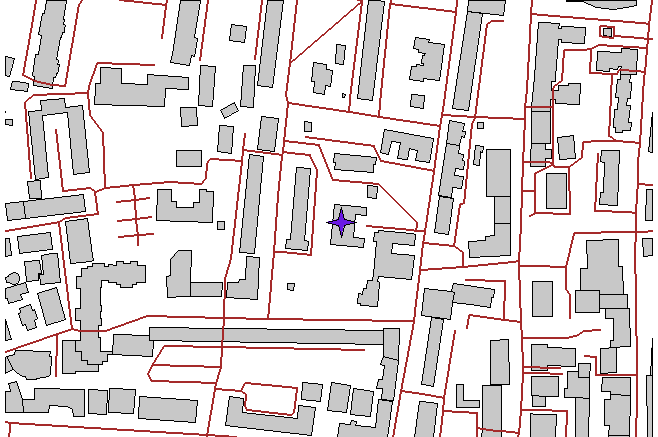
\includegraphics[width=0.6\columnwidth]{./practic/img/area_of_interest.png}
        \end{center}
    \end{figure}
    На карте представлены:
    \begin{itemize}
        \item Здания (buildings): серые многоугольники
        \item Дороги (roads): красные линии
        \item Объект, тоступность которого измеряется обозначен синей звездой (mypoint).
    \end{itemize}

\end{frame}

\begin{frame}
    \frametitle{Решение на базе векторного подхода: идея}
    Общий план действий:
    \begin{enumerate}
        \item Строим топологически корректный граф дорог и присоединяем к нему точку, для которой будем оценивать зоны доступности.
        \item Делим полученный граф дорог на зоны доступности.
    \end{enumerate}
\end{frame}

\begin{frame}[allowframebreaks,fragile]
    \frametitle{Решение на базе векторного подхода: реализация}
    \begin{enumerate}
        \item Строим топологически корректный граф дорог и присоединяем к нему точку, для которой будем оценивать зоны доступности:
        \begin{enumerate}
            \item В ходе векторизации дороги могли быть построены так, что они пересекаются визуально, но общей вершины у них нет. Воспользуемся инструментом v.clean, чтобы добавить общие вершины:
            \begin{verbatim}
v.clean in=roads out=roads_br
    tool=snap,break,rmdupl thre=0.5,0,0
            \end{verbatim}
            здесь мы <<прищелкнули>> вершины друг к другу, если они лежат ближе, чем 0.5 метра, затем разбили линии в точках пересечения (добавили к ним вершины) и удалили возможные дубликаты линий. В результате был получен новый векторный слой roads\_br.
            \item Создадим граф дорог (roads\_network), добавив к нему точки из слоя mypoint (присоединим точки, если они лежат на расстоянии от дорог меньшем, чем 10 километров):
            \begin{verbatim}
v.net input=roads_br points=mypoint
    output=road_network
    operation=connect thresh=10000
            \end{verbatim}
            Результат показан на рисунке (заметим на будущее, что точка была присоеденена к дороге, проходящей к востоку от нее):
            \begin{figure}[!ht]
                \begin{center}
                    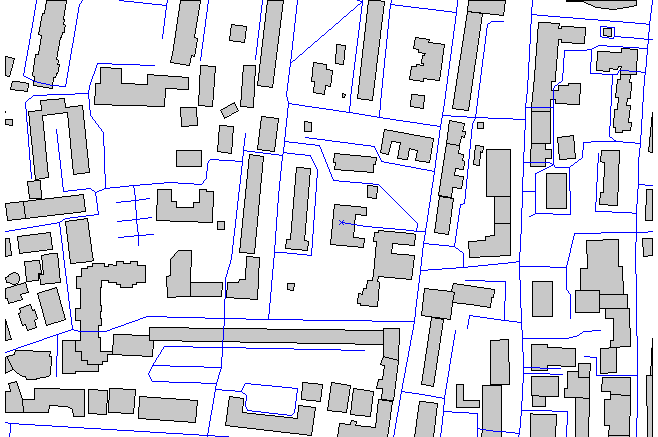
\includegraphics[width=0.8\columnwidth]{./practic/img/roads_network}
                \end{center}
            \end{figure}
        \end{enumerate}
        \item Делим полученный граф дорог на зоны доступности, которые будем рассчитывать для точек с категориями от 1 до 1000000 (здесь берем категории с запасом; можно указать категории конкретных точек) слоя road\_network:
        \begin{verbatim}
v.net.iso input=road_network
    output=road_network_iso
    ccats=1-1000000 costs=250
            \end{verbatim}
    \end{enumerate}
    Построенный граф road\_network\_iso содержит два типа линий: категория 1 -- линии, которые лежат ближе, чем 250 метров и категория 2 --- линии, которые лежат далее, чем 250 метров (можно было разбить граф на большее число категорий). Результат показан на рисунке:
            \begin{figure}[!ht]
                \begin{center}
                    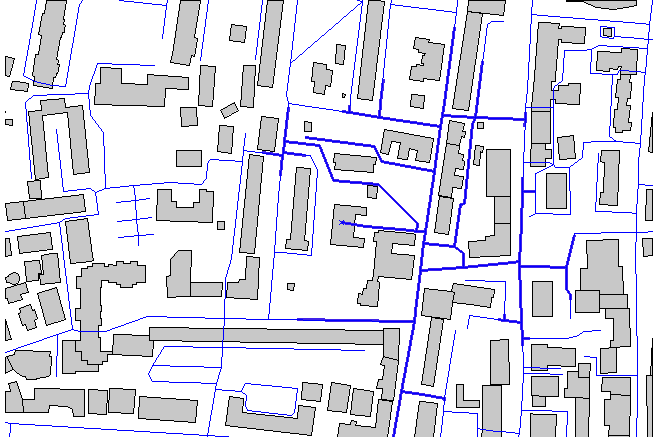
\includegraphics[width=0.9\columnwidth]{./practic/img/roads_iso}
                \end{center}
                \caption{Зоны доступности}
            \end{figure}
    Как видим, зона доступности к западу от точки значительно меньше, чем к востоку (вспомним, что точка была присоеденена к дороге, проходящей к востоку от нее), хотя расстояние от точки до ближайшей западной дороги было лишь незначительно больше, чем до ближайшей восточной.
\end{frame}

\begin{frame}
    \frametitle{Замечания}
    \begin{itemize}
        \item Мы строили граф дорог и расчитывали по нему расстояния, используя в качестве веса ребра графа его длину в географическом пространстве. GRASS позволяет использовать таблицу аттрибутов для назначения веса ребрам графа.
        \item Мы считали, что движение по дорогам может идти в обоих направлениях. При необходимости можно указать что ребра графа являются однонаправленными.
    \end{itemize}
    Более подробную информацию об этих и других параметрах модулей см. в документации.
\end{frame}


\begin{frame}
    \frametitle{Решение на базе растрового подхода: идея}
    Общий план действий:
    \begin{enumerate}
        \item Построим растр стоимости движения, который будет показывать, насколько сложно пройти через ячейку: если ячейка принадлежит зданию, цена прохода будет очень большой, если же проход через ячейку свободен, то назначим цену прохода через нее равным ширине (высоте) ячейки.
        \item Запустим процедуру поиска доступности заданной точки, используя растр стоимости. В результате будет найден растр суммарной цены прохода: в ячеке растра будет храниться цена передвижения от ячейки до точки.
        \item (Опционально) Построим полигоны, соответствующие зонам доступности.
    \end{enumerate}
\end{frame}

\begin{frame}[fragile,allowframebreaks]
    \frametitle{Решение на базе растрового подхода: реализация}
    \begin{enumerate}
        \item Построение растра стоимости.
        \begin{enumerate}
            \item Зададим размер ячейки растра равным одному метру:
            \begin{verbatim}
g.region res=1 -p
            \end{verbatim}
            \item Растеризуем здания, указав, что ячейки, лежащие под зданиями должны иметь большое значение (10000):
            \begin{verbatim}
v.to.rast in=buildings_aoi
    out=buildings_aoi use=val val=10000
            \end{verbatim}
            \item Построим растр стоимости:
            \begin{verbatim}
r.mapcalc "cost=1"
r.mapcalc "cost=
    if(isnull(buildings_aoi),
        cost, buildings_aoi)"
            \end{verbatim}
            \item Растеризуем точки (точка может попасть на здание, как и в нашем случае, поэтому увеличим ее размер, чтобы она вышла за пределы здания):
            \begin{verbatim}
v.to.rast mypoint out=mypoint use=val val=1
r.grow mypoint out=point radius=10
            \end{verbatim}
            \item Впечатаем точку в растр стоимости, чтобы она <<прорезала>> здание:
            \begin{verbatim}
r.mapcalc "cost=if(isnull(point), cost, point)"
            \end{verbatim}
            Растр стоимости показан на рисунке:
            \begin{figure}[!ht]
                \begin{center}
                    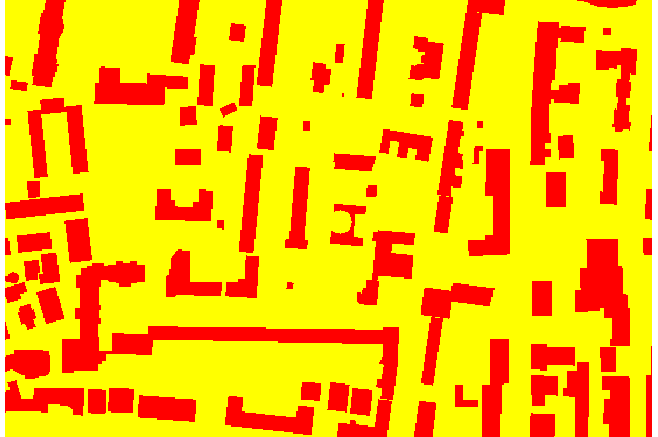
\includegraphics[width=0.8\columnwidth]{./practic/img/cost}
                \end{center}
                \caption{Стоимость движения через ячейки (красный цвет --- 10000, желтый --- 1)}
            \end{figure}
        \end{enumerate}
        \item Зоны доступности:
        \begin{enumerate}
            \item Построим растр суммарной стоимости движения
            \begin{verbatim}
r.cost -k in=cost output=distance
    start_point=mypoint max_cost=250
r.mapcalc "distance =
    if(distance<=250, distance, null())"
            \end{verbatim}
            В последней команде мы удаляем из растра все ячейки, стомость пути до которых превышает 250.
            \begin{figure}[!ht]
                \begin{center}
                    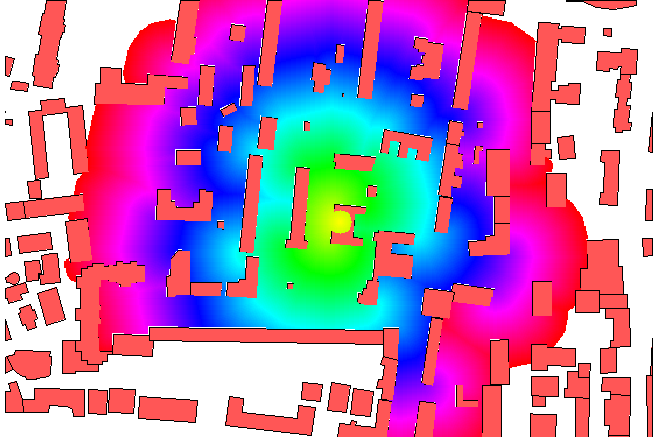
\includegraphics[width=0.8\columnwidth]{./practic/img/cum_cost}
                \end{center}
                \caption{Суммарная стоимость движения от точки mypoint}
            \end{figure}
            \item Построим векторные изолинии стоимости движения шагом 50 метров:
            \begin{verbatim}
r.mapcalc "iso_dist = 50 *int(distance/50)"
r.to.vect in=iso_dist out=distance feature=area
            \end{verbatim}
            Результат показан на рисунке:
            \begin{figure}[!ht]
                \begin{center}
                    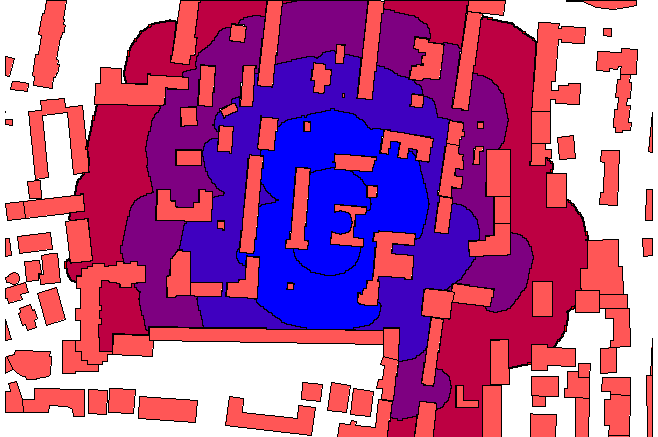
\includegraphics[width=0.8\columnwidth]{./practic/img/vector_cum_cost}
                \end{center}
                \caption{Изолинии стоимости движения от точки mypoint}
            \end{figure}
        \end{enumerate}
    \end{enumerate}
\end{frame}

\begin{frame}[fragile,allowframebreaks]
    \frametitle{Дополнительный пример}
    В предыдущем примере стоимость движения была одинакова во всех направлениях, наличие дорог не учитывалось. Можно учесть, что
    по дороге идти легче (допустим в два раза), тогда:
    \begin{verbatim}
g.region res=1 -p
v.to.rast in=buildings_aoi
    out=buildings_aoi use=val val=10000
v.to.rast roads out=roads use=val val=1

r.mapcalc "cost=2"  # пустое место
r.mapcalc "cost=
    if(isnull(buildings_aoi), cost, buildings_aoi)"
r.mapcalc "cost=
    if(isnull(roads), cost, roads)"

v.to.rast mypoint out=mypoint use=val val=1
r.grow mypoint out=point radius=10
r.mapcalc "cost=if(isnull(point), cost, point)"

r.cost -k in=cost output=distance
    start_point=mypoint max_cost=250
r.mapcalc "distance =
    if(distance<=250, distance, null())"
    \end{verbatim}
    \begin{figure}[!ht]
        \begin{center}
            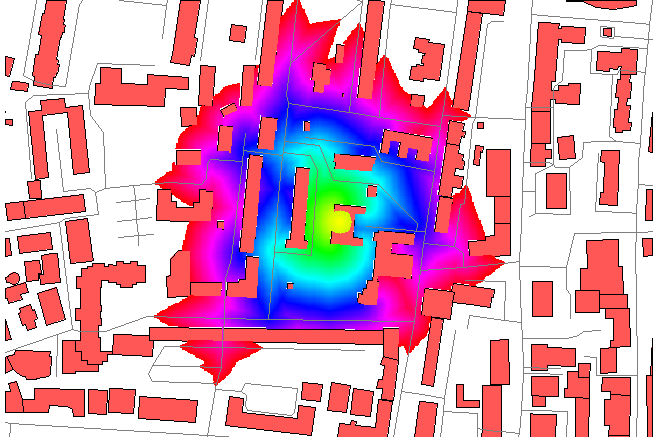
\includegraphics[width=0.9\columnwidth]{./practic/img/cum_cost2}
        \end{center}
        \caption{Суммарная стоимость движения от точки mypoint с учетом дорог}
    \end{figure}
\end{frame}

